\documentclass{standalone}
\usepackage{tikz}
\begin{document}
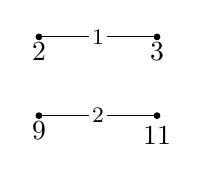
\begin{tikzpicture}[every node/.style={draw, circle, fill=black, minimum size=2pt, inner sep=0pt}]
\node[fill=black, label=below:{$2$}] (G1N1) at (6,4.5) {};
\node[fill=black, label=below:{$3$}] (G1N0) at (7.5,4.5) {};
\node[fill=black, label=below:{$9$}] (G1N2) at (6,3.5) {};
\node[fill=black, label=below:{$11$}] (G1N3) at (7.5,3.5) {};
\draw (G1N0) -- (G1N1) node (m) [midway, draw =none, fill=white] {\footnotesize$1$};
\draw (G1N3) -- (G1N2) node (m) [midway, draw =none, fill=white] {\footnotesize$2$};
\end{tikzpicture}
\end{document}
